\documentclass[12pt]{article}

\usepackage{tikz} % картинки в tikz
\usepackage{microtype} % свешивание пунктуации
\usepackage{array} % для столбцов фиксированной ширины
\usepackage{comment} % для комментирования целых окружений
\usepackage{indentfirst} % отступ в первом параграфе

\usepackage{sectsty} % для центрирования названий частей
\allsectionsfont{\centering}

\usepackage{amsmath, amssymb, amsthm, amsfonts} % куча стандартных математических плюшек

\usepackage[top=2cm, left=1cm, right=1cm, bottom=2cm]{geometry} % размер текста на странице
\usepackage{lastpage} % чтобы узнать номер последней страницы
 
\usepackage{enumitem} % дополнительные плюшки для списков
%  например \begin{enumerate}[resume] позволяет продолжить нумерацию в новом списке

\usepackage{caption} % подписи к рисункам
\usepackage{hyperref} % гиперссылки
\usepackage{multicol} % текст в несколько столбцов


\usepackage{fancyhdr} % весёлые колонтитулы
\pagestyle{fancy}
\lhead{Введение в машинное обучение, ВШЭ}
\chead{}
\rhead{2022-06-24}
\lfoot{Вариант $\Sigma \Theta \Kappa$}
\rfoot{Паниковать запрещается!}
%\rfoot{Тест}
\renewcommand{\headrulewidth}{0.4pt}
\renewcommand{\footrulewidth}{0.4pt}

\usepackage{ifthen} % для написания условий

\usepackage{todonotes} % для вставки в документ заметок о том, что осталось сделать
% \todo{Здесь надо коэффициенты исправить}
% \missingfigure{Здесь будет Последний день Помпеи}
% \listoftodos --- печатает все поставленные \todo'шки


% более красивые таблицы
\usepackage{booktabs}
% заповеди из докупентации:
% 1. Не используйте вертикальные линни
% 2. Не используйте двойные линии
% 3. Единицы измерения - в шапку таблицы
% 4. Не сокращайте .1 вместо 0.1
% 5. Повторяющееся значение повторяйте, а не говорите "то же"


\usepackage{fontspec}
\usepackage{polyglossia}

\setmainlanguage{russian}
\setotherlanguages{english}

% download "Linux Libertine" fonts:
% http://www.linuxlibertine.org/index.php?id=91&L=1
\setmainfont{Linux Libertine O} % or Helvetica, Arial, Cambria
% why do we need \newfontfamily:
% http://tex.stackexchange.com/questions/91507/
\newfontfamily{\cyrillicfonttt}{Linux Libertine O}

% Математические шрифты 
% Математические шрифты 
\usepackage{unicode-math}     
\setmathfont[math-style=upright]{euler.otf} 

\setmathfont[range={\mathbb, \mathop, \heartsuit, \angle, \smile, \varheartsuit}]{Asana-Math.otf}

\AddEnumerateCounter{\asbuk}{\russian@alph}{щ} % для списков с русскими буквами
\setlist[enumerate, 2]{label=\asbuk*),ref=\asbuk*}


% мои цвета https://www.artlebedev.ru/colors/
\definecolor{titleblue}{rgb}{0.2,0.4,0.6} 
\definecolor{blue}{rgb}{0.2,0.4,0.6} 
\definecolor{red}{rgb}{1,0,0.2} 
\definecolor{green}{rgb}{0,0.6,0} 
\definecolor{purp}{rgb}{0.4,0,0.8} 

% цвета из geogebra 
\definecolor{litebrown}{rgb}{0.6,0.2,0}
\definecolor{darkbrown}{rgb}{0.75,0.75,0.75}

% Гиперссылки
\usepackage{xcolor}   % разные цвета

\usepackage{hyperref}
\hypersetup{
  unicode=true,           % позволяет использовать юникодные символы
  colorlinks=true,        % true - цветные ссылки
  urlcolor=blue,          % цвет ссылки на url
  linkcolor=black,          % внутренние ссылки
  citecolor=green,        % на библиографию
  breaklinks              % если ссылка не умещается в одну строку, разбивать её на две части?
}

% эпиграфы
\usepackage{epigraph}
\setlength\epigraphwidth{.5\textwidth}
\setlength\epigraphrule{0pt}

% Математические операторы первой необходимости:
\DeclareMathOperator{\sgn}{sign}
\DeclareMathOperator*{\argmin}{arg\,min}
\DeclareMathOperator*{\argmax}{arg\,max}
\DeclareMathOperator{\Cov}{Cov}
\DeclareMathOperator{\Var}{Var}
\DeclareMathOperator{\Corr}{Corr}
\DeclareMathOperator{\E}{\mathop{E}}
\DeclareMathOperator{\Med}{Med}
\DeclareMathOperator{\Mod}{Mod}
\DeclareMathOperator*{\plim}{plim}

\DeclareMathOperator{\logloss}{logloss}
\DeclareMathOperator{\softmax}{softmax}

\DeclareMathOperator{\tr}{tr}

% команды пореже
\newcommand{\const}{\mathrm{const}}  % const прямым начертанием
\newcommand{\iid}{\sim i.\,i.\,d.}  % ну вы поняли...
\newcommand{\fr}[2]{\ensuremath{^{#1}/_{#2}}}   % особая дробь
\newcommand{\ind}[1]{\mathbbm{1}_{\{#1\}}} % Индикатор события
\newcommand{\dx}[1]{\,\mathrm{d}#1} % для интеграла: маленький отступ и прямая d

% одеваем шапки на частые штуки
\def \hb{\hat{\beta}}
\def \hs{\hat{s}}
\def \hy{\hat{y}}
\def \hY{\hat{Y}}
\def \he{\hat{\varepsilon}}
\def \hVar{\widehat{\Var}}
\def \hCorr{\widehat{\Corr}}
\def \hCov{\widehat{\Cov}}

% Греческие буквы
\def \a{\alpha}
\def \b{\beta}
\def \t{\tau}
\def \dt{\delta}
\def \e{\varepsilon}
\def \ga{\gamma}
\def \kp{\varkappa}
\def \la{\lambda}
\def \sg{\sigma}
\def \tt{\theta}
\def \Dt{\Delta}
\def \La{\Lambda}
\def \Sg{\Sigma}
\def \Tt{\Theta}
\def \Om{\Omega}
\def \om{\omega}

% Готика
\def \mA{\mathcal{A}}
\def \mB{\mathcal{B}}
\def \mC{\mathcal{C}}
\def \mE{\mathcal{E}}
\def \mF{\mathcal{F}}
\def \mH{\mathcal{H}}
\def \mL{\mathcal{L}}
\def \mN{\mathcal{N}}
\def \mU{\mathcal{U}}
\def \mV{\mathcal{V}}
\def \mW{\mathcal{W}}

% Жирные буквы
\def \mbb{\mathbb}
\def \RR{\mbb R}
\def \NN{\mbb N}
\def \ZZ{\mbb Z}
\def \PP{\mbb{P}}
\def \QQ{\mbb Q}

\def \putyourname{\fbox{
    \begin{minipage}{42em}
      Фамилия, имя, номер группы:\vspace*{3ex}\par
      \noindent\dotfill\vspace{2mm}
    \end{minipage}
  }
}

\def \checktable{

  \vspace{5pt}
  Табличка для проверяющих работу:

\vspace{5pt}

  \begin{tabular}{|m{2cm}|m{1cm}|m{1cm}|m{1cm}|m{1cm}|m{1cm}|m{1cm}|m{1cm}|m{2cm}|}
\toprule
    Вопрос & 11 &  12 & 13 & 14 & 15 & 16 & 17 & Итого \\
\midrule
    Баллы &  &  & & & & & &  \\
 \bottomrule
\end{tabular}
}


\def \testtable{

\vspace{5pt}
  Внесите сюда ответы на тест:

\vspace{5pt}

\begin{tabular}{|m{2cm}|m{0.6cm}|m{0.6cm}|m{0.6cm}|m{0.6cm}|m{0.6cm}|m{0.6cm}|m{0.6cm}|m{0.6cm}|m{0.6cm}|m{0.6cm}|}
\toprule
    Вопрос & 1 &  2 & 3 & 4 & 5 & 6 & 7 & 8 & 9 & 10 \\
\midrule
    Ответ &  &  & & & & & & & & \\
 \bottomrule
\end{tabular}
}


% [1][3] 1 = one argument, 3 = value if missing
% эта магия создаёт окружение answerlist
% именно в окружении answerlist записаны варианты ответов в подключаемых exerciseXX
% просто \begin{answerlist} сделает ответы в три столбца
% если ответы длинные, то надо в них руками сделать
% \begin{answerlist}[1] чтобы они шли в один столбец
\newenvironment{answerlist}[1][3]{
\begin{multicols}{#1}

\begin{enumerate}[label=\fbox{\emph{\Alph*}},ref=\emph{\alph*}]
}
{
\item Нет верного ответа.
\end{enumerate}
\end{multicols}
}

% BB: unicol version. don't know why \ifthenelse fails in second part of new-env
\newenvironment{answerlistu}{
\begin{enumerate}[label=\fbox{\emph{\Alph*}},ref=\emph{\alph*}]
}
{
\item Нет верного ответа.
\end{enumerate}
}


\excludecomment{solution} % without solutions

\theoremstyle{definition}
\newtheorem{question}{Вопрос}

\usepackage{tikzlings}
\usepackage{tikzducks}

\usepackage{alltt}

\begin{document}

\putyourname

\testtable

\checktable

\mbox{ }

\epigraph{«Если орел — я выиграла, если решка — ты проиграл»
}{\textit{Рейчел Грин, сериал "Друзья"}}

Работа состоит из трёх частей: тестовая, задачи и ответы на открытые вопросы. Работа пишется на раздаточном материале. Черновики можно использовать, но не сдавать - их не проверяем.
Списывание карается обнулением работы. Удачи!

\section*{Часть первая: тестовая} 

Дайте ответ на $10$ тестовых вопросов. Каждый вопрос стоит $3$ балла. Никаких дополнительных пояснений в этой части работы от вас не требуются.
\begin{question}
В листьях деревьев записаны
\begin{answerlist}
  \item предикаты
  \item прогнозы
  \item вопросы
  \item условные выражения
  \item критерии информативности
\end{answerlist}
\end{question}

\begin{question}
Выберите верное утверждение про измерение энтропии при разбиении вершины
\begin{answerlist}
  \item Энтропия считается для распределения признаков в вершине.
  \item Разумно выбирать разбиения, при котором энтропия в дочерних вершинах как можно больше.
  \item Чем меньше энтропия в вершине, тем больше элементов одного класса в вершине.
  \item Энтропия не используется для разбиения вершин.
  \item Высокая энтропия в вершине - критерий останова обучения.
\end{answerlist}
\end{question}

\begin{question}
Джо, Чендлер и Росс выписывали недостатки алгоритмов. Какой недостаток они указали для решающих деревьев?
\begin{answerlist}
  \item Необходимость масштабирования признаков.
  \item Работа с ограниченным объемом данных.
  \item Работа с ограниченными типами данных.
  \item Долгое обучение.
  \item Склонность к переобучению.
\end{answerlist}
\end{question}

\begin{solution}
\begin{answerlist}
  \item Good answer :)
  \item Bad answer :(
  \item Bad answer :(
  \item Bad answer :(
  \item Bad answer :(
\end{answerlist}
\end{solution}

\begin{question}
Ошибка модели складывается из
\begin{answerlist}
  \item трех компонент: шума, смещения и разброса.
  \item двух компонент: смещения и разброса.
  \item двух компонент: шума и разброса.
  \item трех компонент: шума, смещения и матожидания.
  \item трех компонент: матожидания, смещения и разброса.

\end{answerlist}
\end{question}

\begin{question}
Выберите утверждение, которое неверно для случайного леса
\begin{answerlist}
  \item Базовые алгоритмы обучаются на бутстрапированной выборке.
  \item При разбиении узла используются все признаки.
  \item При обучении базового алгоритма могут использоваться одни и те же объекты.
  \item Алгоритмы обучаются независимо друг от друга.
  \item Базовые алгоритмы представляют собой неглубокие деревья.
\end{answerlist}
\end{question}

\begin{question}
Выберите одно верное утверждение
\begin{answerlist}
  \item Решающие деревья устойчивы к изменениям в выборке.
  \item Случайный лес имеет меньшее смещение, чем решающее дерево той же глубины.
  \item Разброс случайного леса выше, чем решающего дерева той же глубины.
  \item Добавление дерева в лес уменьшает ошибку в N раз.
  \item Оценить качество случайного леса можно без тестовой выборки.

\end{answerlist}
\end{question}

\begin{question}
Обучение без учителя, в отличие от обучения с учителем
\begin{answerlist}
  \item предполагает наличие целевой переменной.
  \item предполагает наличие тестовой выборки.
  \item не предполагает наличие целевой переменной.
  \item предполагает наличие валидационной выборки.
  \item не предполагает наличие тестовой выборки.
\end{answerlist}
\end{question}

\begin{question}
Выберите верное утверждение про DBSCAN.
\begin{answerlist}
  \item Метод зависит от расположения центров кластера.
  \item Метод может не сойтись.
  \item Методу нужные правильные ответы для обучения.
  \item Метод сам определяет количество кластеров.
  \item Метод поделит на K кластеров, K надо задать заранее.
\end{answerlist}
\end{question}


\begin{question}
PCA - это алгоритм для
\begin{answerlist}
  \item регрессии.
  \item классификации.
  \item понижения размерности.
  \item кластеризации.
  \item рекомендательных систем.
\end{answerlist}
\end{question}

\begin{question}
Джо не делится едой, поэтому Чендлер 5 дней заказывал то же, что и Джо, чтобы понять его вкус. 1 - если еда понравилась, 0 - если нет.
\begin{table}[h]
    \centering
    \begin{tabular}{>{\bfseries}cccccccc}
        \toprule
         Джо & $1$ & $1$ & $1$ & $1$ & $1$  \\ \midrule
         Чендлер & $1$ & $0$ & $1$ & $1$ & $0$ \\
         \bottomrule
    \end{tabular}
\end{table}
Если на Джо смотреть как на рекомендательную систему, чему ему равен p@5 для Чендлера?
\begin{answerlist}
  \item 0.2
  \item 0.6
  \item 0.4
  \item 0.8
  \item 0.5
\end{answerlist}
\end{question}
\newpage 

\section*{Часть вторая: открытые вопросы}

Эта часть состоит из открытых вопросов. На них необходимо дать краткие, но ёмкие ответы. За каждый ответ вы можете получить до 10 баллов.


\begin{question}
Опишите пошагово, как обучается градиентный бустинг для произвольной функции потерь. Фиби планирует написать научно-просветительскую песню, и ей очень нужные доходчивые объяснения. 
\end{question}

\vspace{7cm} 


\begin{question}
Чендлер задумался о композициях над решающими деревьями. Допустим, думает он, мы обучили две композиции решающих деревьев: случайный лес и градиентный бустинг. В обоих случаях мы остановили добавление деревьев, когда ошибка на валидационной выборке перестала убывать. Что произойдёт с ошибкой этих моделей на валидационной выборке, если мы продолжим обучение и добавим в каждую из них по 10 000 деревьев? Обоснуйте ваш ответ.
\end{question}

\newpage


\begin{question}
Рейчел прочитала про алгоритм K-means и решила использовать его для сортировки вещей на складе модного дома, где она работает, но не знает, на сколько кластеров разбить данные. Как подобрать оптимальное число кластеров в алгоритме K-means? Опишите подробно метод.

\end{question}


\vspace{10cm} 

\begin{question}
Джо пытается найти новую работу и пользуется сервисом по подбору вакансий, которые используют рекомендательные системы для подборки подходящих вакансий.
Как работает коллаборативная фильтрация? Какие виды коллаборативной фильтрации вы знаете? Опишите, как работают известные вам подходы.

\end{question}
\newpage 

\begin{question}
Моника со скрупулезностью разрабатывает новый рецепт. Чтобы успокоить нервы, она обучает модели машинного обучения в перерывах. На картинке представлены 4 регрессионных дерева, обученных на одних и тех же данных. Варьируется один гиперпараметр. Какой гиперпараметр это может быть? Предположите, какие значения гиперпараметра могут соответствовать каждой картинке. К чему приводит очень большое значение этого гиперпараметра? Предположите, какое значение и картинку стоит выбрать.
\begin{center}
    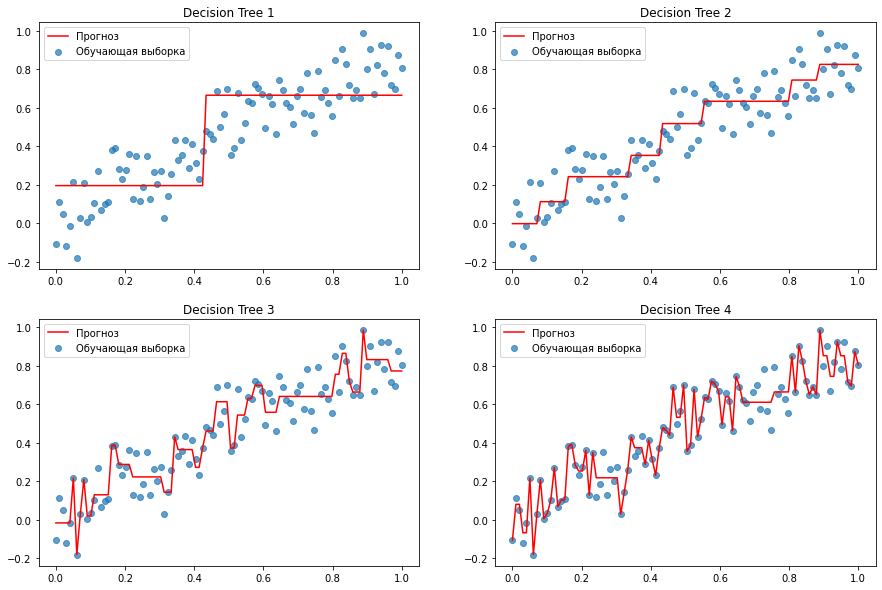
\includegraphics[scale=0.5]{tree_depth_var2.png}
\end{center}
\end{question}




\newpage 


\section*{Часть третья: задачки}

Решите все задания. Все ответы должны быть обоснованы. Решения должны быть прописаны для каждого пункта. Рисунки должны быть чёткими и понятными. Все линии должны быть подписаны. За решение каждой задачи вы можете получить до 10 баллов.


\begin{question}
Гантер утомился видеть постоянно бездельничающих друзей на диване и решил себя развлечь, записывая, сколько чашек кофе они заказывают в неделю. $y$  - количество чашек кофе, $x_1$ - присоединился ли Росс к друзьям или нет,   $x_2$ - погода в градусах по Цельсию.

Гантер построил решающее дерево, прогнозирующее количество заказанных чашек кофе, и хотел было применить его, но Рейчел разлила на листок с деревом кофе. Помогите Гантеру восстановить дерево.
 
 Дерево строится до идеального прогноза. В качестве критерия для разбиения узла Гантер использовал MSE.

\begin{center}
    \begin{tabular}{ccc}
        \toprule
        $y$ & $x_1$ & $x_2$ \\
        \midrule
        $12$ & $0$ & $5$ \\
        $3$ & $1$ & $6$ \\
        $6$ & $1$ & $7$ \\
        $9$ & $1$ & $8$\\
        $18$ & $0$ & $12$ \\
        $21$ & $0$ & $13$ \\
        \bottomrule
    \end{tabular}
\end{center}
\end{question}


\newpage 

\begin{question}
Росс задумался, можно ли поделить посетителей кофейни Central Perk на кластеры. В статье он прочитал, что алгоритм DBSCAN получил в этом году премию. Он решил использовать его с параметрами eps=2 и minsamples=1, чтобы выделить кластеры.

Росс пришел к вам за проверкой своих изысканий. Кластеризуйте точки по алгоритму DBSCAN с заданными параметрами.

Сколько кластеров получилось?
\begin{center}
    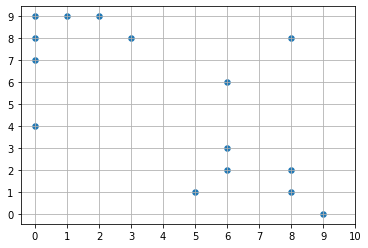
\includegraphics[scale=0.5]{dbscan_var2.png}
\end{center}

\end{question}

\end{document}
